\documentclass[aspectratio=169, 9pt]{beamer}

\usetheme{Madrid}
\usecolortheme{whale}
\setbeamertemplate{navigation symbols}{}
\setbeamersize{text margin left=4mm, text margin right=4mm}

\usepackage[utf8]{inputenc}
\usepackage[T1]{fontenc}
\usepackage{lmodern}
\usepackage{booktabs}
\usepackage{graphicx}
\usepackage{amsmath,amssymb}
\usepackage{xcolor}
\usepackage{array}
\usepackage{colortbl}

\definecolor{navy}{HTML}{1E293B}
\definecolor{teal}{HTML}{0F766E}
\definecolor{amber}{HTML}{D97706}
\definecolor{crimson}{HTML}{DC2626}
\definecolor{rowgray}{HTML}{F1F5F9}
\definecolor{rowteal}{HTML}{CCFBF1}

\setbeamercolor{palette primary}{bg=navy, fg=white}
\setbeamercolor{palette secondary}{bg=teal, fg=white}
\setbeamercolor{palette tertiary}{bg=navy, fg=white}
\setbeamercolor{frametitle}{bg=navy, fg=white}
\setbeamercolor{block title}{bg=navy, fg=white}
\setbeamercolor{block body}{bg=rowgray, fg=black}
\setbeamercolor{block title alerted}{bg=amber, fg=white}
\setbeamercolor{block body alerted}{bg=rowgray, fg=black}
\setbeamercolor{block title example}{bg=teal, fg=white}
\setbeamercolor{block body example}{bg=rowgray, fg=black}

\setbeamertemplate{footline}{%
  \leavevmode%
  \hbox{%
  \begin{beamercolorbox}[wd=.78\paperwidth,ht=2.25ex,dp=1ex,leftskip=3mm]{author in head/foot}%
    \usebeamerfont{author in head/foot}\textbf{NLP1 Project 1 (Lecture 2a)} $|$ TweetEval 3-Class Sentiment Classification: Tokenizers, Representations, Models \& Bayesian ROPE
  \end{beamercolorbox}%
  \begin{beamercolorbox}[wd=.22\paperwidth,ht=2.25ex,dp=1ex,rightskip=3mm,right]{date in head/foot}%
    Slide \insertframenumber{} / \inserttotalframenumber
  \end{beamercolorbox}}%
  \vskip0pt%
}

\begin{document}

% ==============================================================================
% SLIDE 1: DATASET & EXPLORATORY DATA ANALYSIS (TOPIC 1)
% ==============================================================================
\begin{frame}{1. Dataset \& Exploratory Data Analysis: \texttt{cardiffnlp/tweet\_eval} (Sentiment)}
\vspace{-2mm}
\begin{columns}[T, onlytextwidth]
  \begin{column}{0.48\textwidth}
    \begin{block}{Task \& Official Benchmark Splits ($N = 59,899$ Tweets)}
      \scriptsize
      \begin{itemize}\setlength{\itemsep}{1pt}
        \item \textbf{Task}: 3-class Twitter sentiment ($\mathcal{Y} = \{\text{Neg (0)}, \text{Neu (1)}, \text{Pos (2)}\}$).
        \item \textbf{Challenge}: Short noisy texts ($\approx 18.7$ words/tweet), slang, emojis, hashtags.
      \end{itemize}
      \vspace{0.5mm}
      \centering
      \renewcommand{\arraystretch}{1.05}
      \resizebox{\textwidth}{!}{%
      \begin{tabular}{@{}lrrrr@{}}
        \toprule
        \textbf{Split} & \textbf{Tweets} & \textbf{Neg (0)} & \textbf{Neu (1)} & \textbf{Pos (2)} \\
        \midrule
        Train & $45,615$ & $7,093$ ($15.5\%$) & $20,673$ ($45.3\%$) & $17,849$ ($39.2\%$) \\
        Validation & $2,000$ & $312$ ($15.6\%$) & $869$ ($43.5\%$) & $819$ ($40.9\%$) \\
        \rowcolor{rowteal} \textbf{Test} & $\mathbf{12,284}$ & $\mathbf{3,972}$ ($\mathbf{32.3\%}$) & $\mathbf{5,937}$ ($\mathbf{48.3\%}$) & $\mathbf{2,375}$ ($\mathbf{19.3\%}$) \\
        \bottomrule
      \end{tabular}}
    \end{block}
    \vspace{-1.5mm}
    \begin{alertblock}{Diagnostic Finding: Severe Temporal Prior Shift ($p_{\text{train}}(y) \neq p_{\text{test}}(y)$)}
      \scriptsize
      \begin{itemize}\setlength{\itemsep}{1pt}
        \item \textbf{Prior Shift}: \textbf{Negative} doubles in Test ($15.5\% \to 32.3\%$), while \textbf{Positive} halves ($39.2\% \to 19.3\%$).
        \item \textbf{Why Both Macro-F1 \& Accuracy}: Accuracy alone favors the majority class; \textbf{Macro-F1} ($\frac{1}{3}\sum_{c} F_{1,c}$) weights all 3 classes equally ($1/3$ each). We report \textbf{both} metrics across all CV and Test evaluations.
        \item \textbf{Class-Weighted Loss}: Standard cross-entropy under-predicts Negative; we weight the loss by $w_c = \frac{N}{3 N_c}$ ($\mathbf{2.14}, \mathbf{0.74}, \mathbf{0.85}$).
      \end{itemize}
    \end{alertblock}
  \end{column}
  \begin{column}{0.50\textwidth}
    \centering
    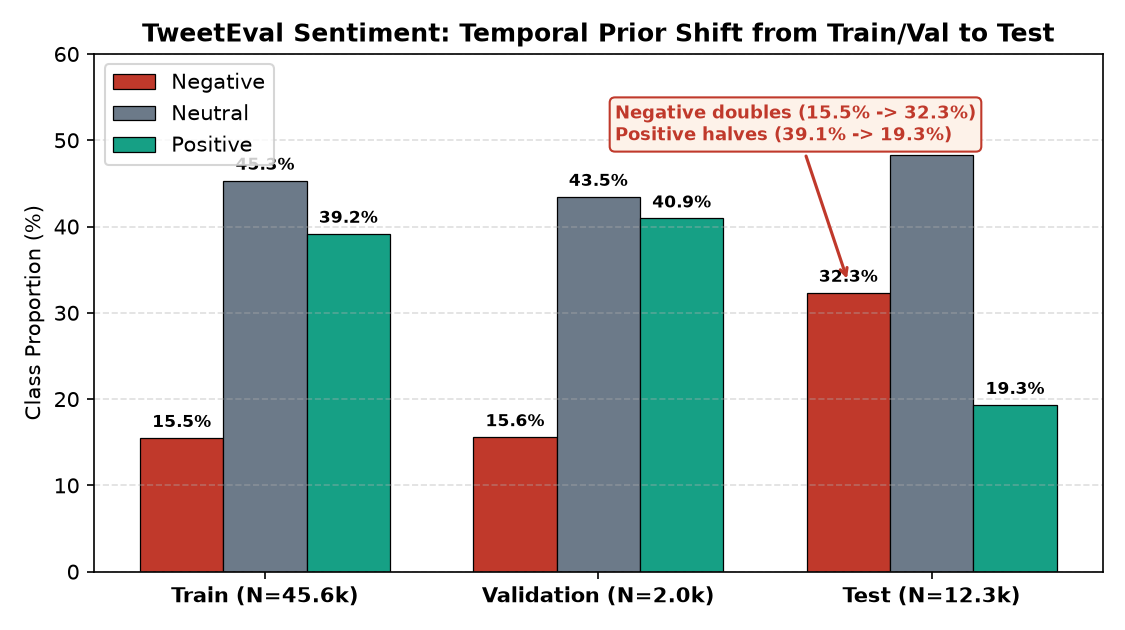
\includegraphics[width=\textwidth]{figures/fig1_class_distribution.png}
  \end{column}
\end{columns}
\end{frame}

% ==============================================================================
% SLIDE 2: TEXT SEGMENTATION & TOKENIZER COMPARISON (TOPIC 2)
% ==============================================================================
\begin{frame}{2. Text Segmentation: Whitespace vs.\ \texttt{TweetTokenizer} vs.\ Subword BPE}
\vspace{-2mm}
\begin{columns}[T, onlytextwidth]
  \begin{column}{0.52\textwidth}
    \begin{block}{Why Do ALL Byte-Level BPE Vocab Sizes Have $0.0\%$ Test OOV?}
      \scriptsize
      \begin{itemize}\setlength{\itemsep}{1pt}
        \item \textbf{Word-Level Tokenizers}: \textbf{Whitespace} ($6.4\%$ Test OOV) glues punctuation (\texttt{"service!"}); \textbf{NLTK \texttt{TweetTokenizer}} ($4.1\%$ Test OOV) uses regex rules for emoticons/handles/elongation (\texttt{"cooool"} $\to$ \texttt{"coool"}).
        \item \textbf{Byte-Level BPE}: Starts its vocabulary with all \textbf{256 single-byte UTF-8 characters}. Any unseen word can always fall back to character pieces $\implies \mathbf{0.0\%}$ \textbf{OOV at every $V$!}
      \end{itemize}
    \end{block}
    \vspace{-2mm}
    \begin{exampleblock}{Concrete Example: Why $V = 8,192$ Is Chosen Over $2\text{k}, 4\text{k}, 16\text{k}$}
      \scriptsize
      Tweet: \texttt{"Unbelievable disappointment!! Literally the worst service \#fail"}\\[1pt]
      \renewcommand{\arraystretch}{1.05}
      \resizebox{\textwidth}{!}{%
      \begin{tabular}{@{}lll@{}}
        \toprule
        \textbf{BPE Vocab $V$} & \textbf{Subword Segmentation (Toks / Tweet)} & \textbf{Effect on Bag-of-Words} \\
        \midrule
        $V = 2,048$ & \texttt{['\_Un','bel','iev','able','\_dis','app','oint','ment',...]} ($37.3$) & Over-splits: \texttt{'bel'}/\texttt{'app'} collide w/ \texttt{'bell'}/\texttt{'apple'}! \\
        $V = 4,096$ & \texttt{['\_Un','believ','able','\_disappoint','ment',...,'f','ail']} ($33.2$) & Still fragments stems (\texttt{'f' + 'ail'}). \\
        \rowcolor{rowteal} $\mathbf{V = 8,192}$ & \texttt{\textbf{['\_Un','believable','\_disappointment','!!',...,'\#','fail']}} ($\mathbf{29.6}$) & \textbf{Sweet Spot}: Keeps full sentiment roots intact! \\
        $V = 16,384$ & \texttt{['\_Unbelievable','\_disappointment',...,'\_\#fail']} ($27.6$) & Memorizes rare tags; \textbf{doubles model params ($2\times$)}! \\
        \bottomrule
      \end{tabular}}
    \end{exampleblock}
  \end{column}
  \begin{column}{0.46\textwidth}
    \centering
    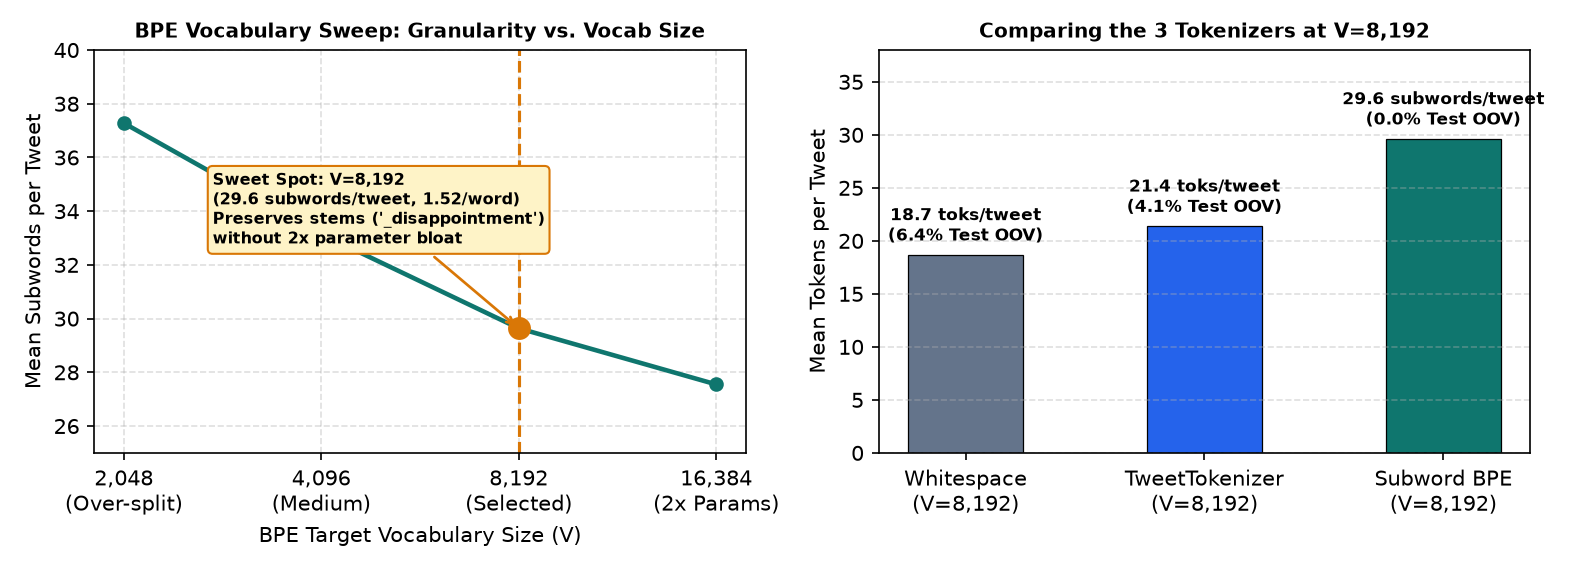
\includegraphics[width=\textwidth]{figures/fig2_tokenizer_comparison.png}
  \end{column}
\end{columns}
\end{frame}

% ==============================================================================
% SLIDE 3: DOCUMENT REPRESENTATIONS (TOPIC 3)
% ==============================================================================
\begin{frame}{3. Document Representations: Token Indicators, Bag-of-Words \& TF-IDF}
\vspace{-2mm}
\begin{columns}[T, onlytextwidth]
  \begin{column}{0.53\textwidth}
    \begin{block}{Three Unigram Feature Functions $h: \mathcal{X} \to \mathbb{R}^{8,192}$ (Lecture 2a)}
      \scriptsize
      \begin{enumerate}\setlength{\itemsep}{1pt}
        \item \textbf{Token Indicators (Binary)}: $h_i^{\text{ind}}(x) = \mathbb{I}(\text{token } i \in x) \in \{0, 1\}$.
        \item \textbf{Bag-of-Words (Counts in Tweet)}: $h_i^{\text{bow}}(x) = \text{tf}(i, x) \in \{0, 1, 2, \dots\}$.
        \item \textbf{Unigram TF-IDF (Our Extension)}: Computed on \textbf{unigram BPE tokens}:
        \begin{itemize}\scriptsize\setlength{\itemsep}{0pt}
          \item $\text{tf}(i, x)$ = token count in \textbf{that single tweet $x$}.
          \item $\text{idf}(i) = \log\!\big(\frac{1 + 45,615}{1 + \text{df}(i)}\big) + 1$ across \textbf{all $45,615$ training tweets}.
          \item Divided by the \textbf{single tweet's $L_2$ norm}: $h_i^{\text{tfidf}}(x) = \frac{\text{tf}(i,x)\cdot\text{idf}(i)}{\|\text{tf}(x)\odot\text{idf}\|_2}$.
        \end{itemize}
      \end{enumerate}
    \end{block}
    \vspace{-2mm}
    \begin{exampleblock}{Concrete Vector Example: $x =$ \texttt{"win win win ! the team had a great win"}}
      \scriptsize
      \centering
      \renewcommand{\arraystretch}{1.0}
      \resizebox{\textwidth}{!}{%
      \begin{tabular}{@{}lcccccc@{}}
        \toprule
        \textbf{Token $i$ in Tweet} & \textbf{1.\ Indicator} & \textbf{2.\ BoW (TF)} & \textbf{Dataset $\text{df}(i)$} & \textbf{Dataset $\text{IDF}(i)$} & \textbf{Raw $\text{TF}\times\text{IDF}$} & \textbf{3.\ Final TF-IDF} \\
        \midrule
        \texttt{'the'} (id=12) & $1$ & $1$ & $18,420$ ($40.4\%$) & $1.91$ & $1.91$ & $0.0906$ \\
        \texttt{'great'} (id=205) & $1$ & $1$ & $2,890$ ($6.3\%$) & $3.76$ & $3.76$ & $0.1786$ \\
        \rowcolor{rowteal} \texttt{\textbf{'win'}} \textbf{(id=618)} & $\mathbf{1}$ & $\mathbf{4}$ & $\mathbf{920}$ ($\mathbf{2.0\%}$) & $\mathbf{4.90}$ & $\mathbf{19.61}$ & $\mathbf{0.9317}$ \\
        Other $8,185$ tokens & $0$ & $0$ & --- & --- & $0.00$ & $0.0000$ \\
        \bottomrule
      \end{tabular}}
    \end{exampleblock}
  \end{column}
  \begin{column}{0.45\textwidth}
    \centering
    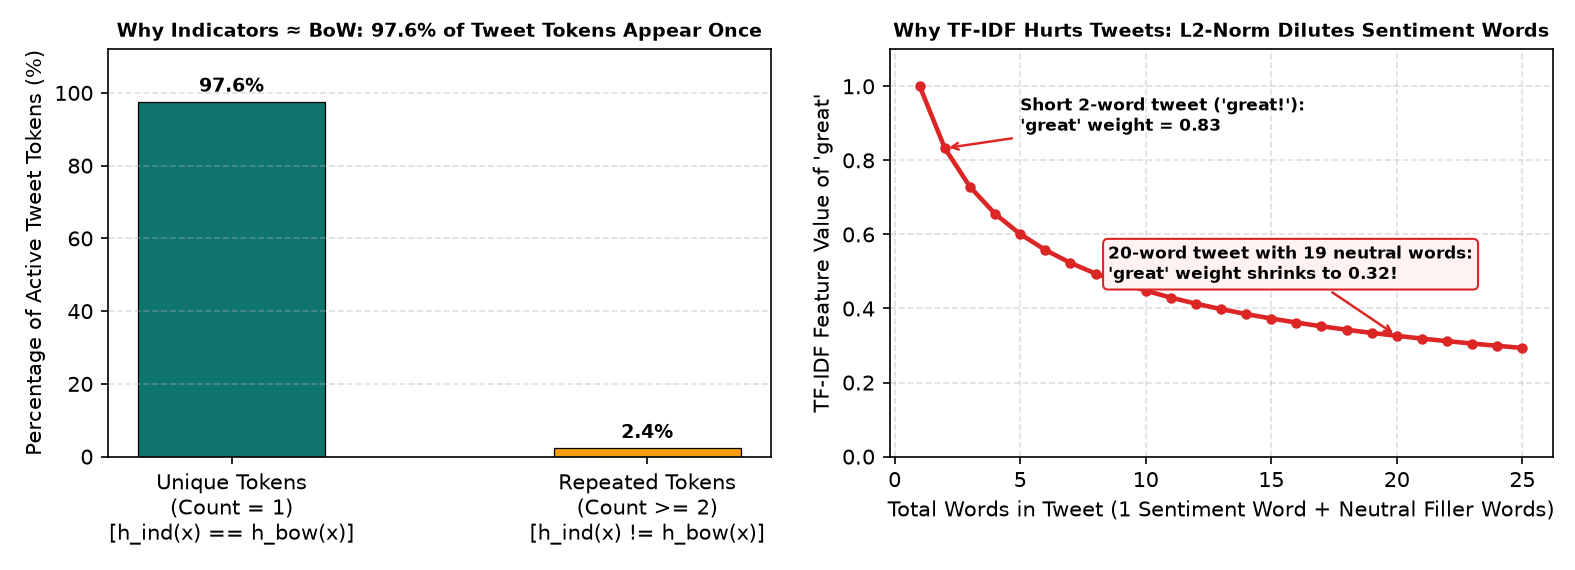
\includegraphics[width=\textwidth]{figures/fig3_representation_diagnostics.png}
  \end{column}
\end{columns}
\end{frame}

% ==============================================================================
% SLIDE 4: MODEL ARCHITECTURES & SOFTMAX REGRESSION (TOPIC 4)
% ==============================================================================
\begin{frame}{4. Model Architectures: Why 98\%+ of MLP Parameters Sit in Layer 1}
\vspace{-2mm}
\begin{columns}[T, onlytextwidth]
  \begin{column}{0.47\textwidth}
    \begin{block}{Softmax Regression Parameterisations (Lecture 2a)}
      \scriptsize
      Given $h(x) \in \mathbb{R}^{8,192}$, each model outputs logits $s(x) \in \mathbb{R}^3$ with $p(y=k|x) = \text{softmax}(s(x))_k$:
      \vspace{1mm}
      \centering
      \renewcommand{\arraystretch}{1.1}
      \resizebox{\textwidth}{!}{%
      \begin{tabular}{@{}lrrr@{}}
        \toprule
        \textbf{Layer / Connection} & \textbf{1.\ Log-Linear} & \textbf{2.\ Shallow MLP} & \textbf{3.\ Deep MLP} \\
        \midrule
        \textbf{Layer 1} ($8,192$-D Input) & $8,192 \times 3 + 3$ & $\mathbf{8,192 \times 256 + 256}$ & $\mathbf{8,192 \times 256 + 256}$ \\
        \quad \textit{Parameters (\% of network)} & $24,579$ ($100\%$) & $\mathbf{2,097,408}$ ($\mathbf{99.96\%}$) & $\mathbf{2,097,408}$ ($\mathbf{98.44\%}$) \\
        \midrule
        \textbf{Layer 2} (Hidden / Out) & --- & $256 \times 3 + 3$ & $256 \times 128 + 128$ \\
        \quad \textit{Parameters (\% of network)} & --- & $771$ ($0.04\%$) & $+32,896$ ($+1.54\%$) \\
        \midrule
        \textbf{Layer 3} (Output) & --- & --- & $128 \times 3 + 3 = 387$ \\
        \midrule
        \rowcolor{rowteal} \textbf{Total Parameters} & $\mathbf{24,579}$ ($\mathbf{1.0\times}$) & $\mathbf{2,098,179}$ ($\mathbf{85.4\times}$) & $\mathbf{2,130,691}$ ($\mathbf{86.7\times}$) \\
        \bottomrule
      \end{tabular}}
    \end{block}
    \vspace{-1.5mm}
    \begin{alertblock}{Why Deep MLP Barely Has More Parameters Than Shallow MLP}
      \scriptsize
      \begin{itemize}\setlength{\itemsep}{1pt}
        \item \textbf{Layer 1 Bottleneck}: Projecting the $8,192$-D vocabulary to $256$ units already costs $\mathbf{2,097,408}$ parameters ($99.96\%$ of Shallow MLP!).
        \item \textbf{Layer 2 ($256 \to 128$)}: Only connects $256$ units to $128$ units ($256 \times 128 + 128 = \mathbf{32,896}$ params, just $+1.5\%$ extra!).
      \end{itemize}
    \end{alertblock}
  \end{column}
  \begin{column}{0.51\textwidth}
    \centering
    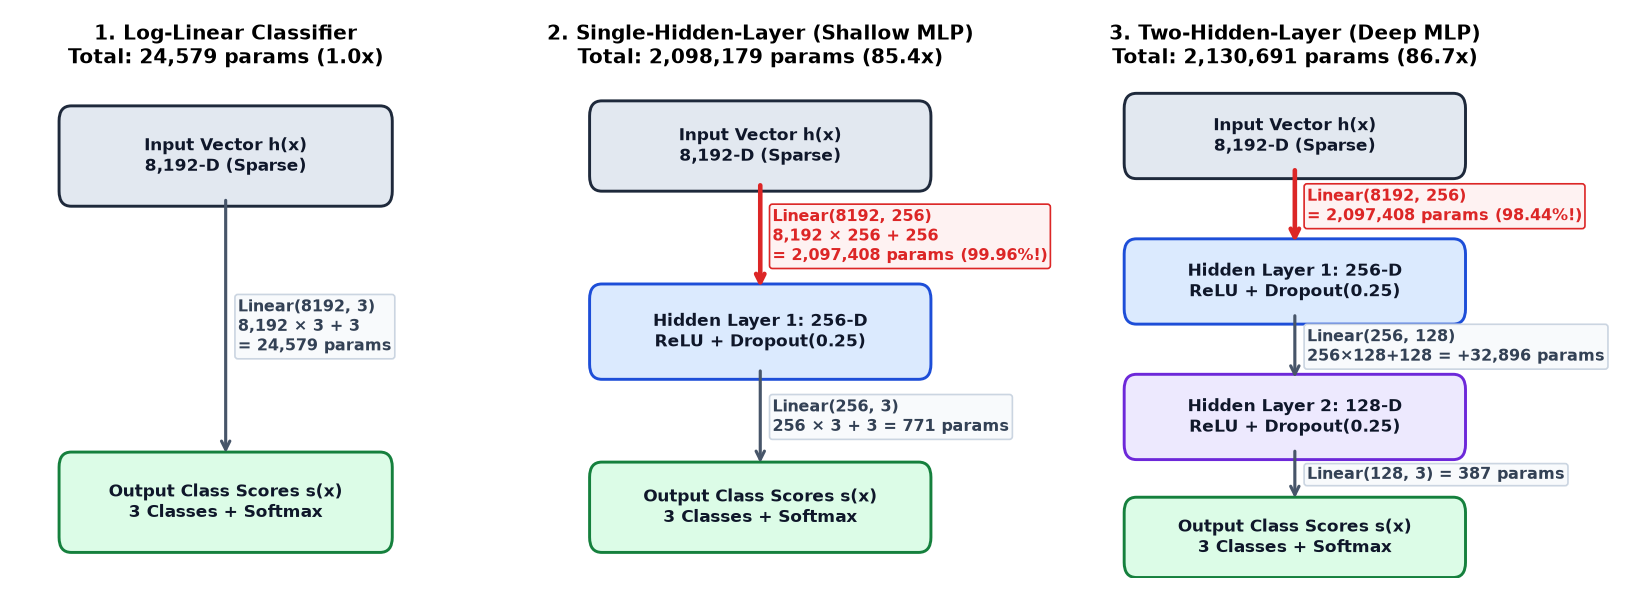
\includegraphics[width=\textwidth]{figures/fig3b_architecture_diagram.png}
  \end{column}
\end{columns}
\end{frame}

% ==============================================================================
% SLIDE 5: 5-FOLD STRATIFIED CV & CORRELATED BAYESIAN ROPE (TOPIC 5)
% ==============================================================================
\begin{frame}{5. 5-Fold Stratified CV \& Correlated Bayesian $t$-Test ($\text{ROPE} = [-0.01, +0.01]$)}
\vspace{-2.5mm}
\begin{columns}[T, onlytextwidth]
  \begin{column}{0.51\textwidth}
    \begin{block}{Exp 5.1: Tokenizer \& BPE Vocab CV (\texttt{BoW} + \texttt{Log-Linear})}
      \scriptsize
      \centering
      \renewcommand{\arraystretch}{0.96}
      \resizebox{\textwidth}{!}{%
      \begin{tabular}{@{}lccc@{}}
        \toprule
        \textbf{Tokenizer} & \textbf{CV Macro-F1} & \textbf{CV Accuracy} & \textbf{Bayesian ROPE vs.\ BPE-8k} \\
        \midrule
        1.\ Whitespace ($V=8\text{k}$) & $0.6091 \pm 0.0051$ & $63.42\% \pm 0.51\%$ & $P(\text{BPE-8k} > \text{WS}) = \mathbf{99.9\%}$ \\
        2.\ \texttt{TweetTokenizer} ($V=8\text{k}$) & $0.6248 \pm 0.0059$ & $64.95\% \pm 0.54\%$ & $P(\text{ROPE}) = \mathbf{100.0\%}$ \\
        3a.\ Subword BPE ($V=2,048$) & $0.6142 \pm 0.0054$ & $63.95\% \pm 0.53\%$ & $P(\text{BPE-8k} > 2\text{k}) = \mathbf{97.6\%}$ \\
        3b.\ Subword BPE ($V=4,096$) & $0.6221 \pm 0.0059$ & $64.68\% \pm 0.55\%$ & $P(\text{ROPE}) = 97.4\%$ \\
        \rowcolor{rowteal} \textbf{3c.\ Subword BPE ($\mathbf{V=8,192}$)} & $\mathbf{0.6263 \pm 0.0062}$ & $\mathbf{65.08\% \pm 0.56\%}$ & \textbf{Selected Sweet Spot} \\
        3d.\ Subword BPE ($V=16,384$) & $0.6258 \pm 0.0061$ & $65.01\% \pm 0.57\%$ & $P(\text{ROPE}) = \mathbf{100.0\%}$ ($2\times$ params) \\
        \bottomrule
      \end{tabular}}
    \end{block}
    \vspace{-2.5mm}
    \begin{block}{Exp 5.2 \& 5.3: Full $3 \times 3$ CV Grid (Tokenizer = BPE $V=8,192$)}
      \scriptsize
      \centering
      \renewcommand{\arraystretch}{0.96}
      \resizebox{\textwidth}{!}{%
      \begin{tabular}{@{}llccc@{}}
        \toprule
        \textbf{Representation} & \textbf{Model} & \textbf{CV Macro-F1} & \textbf{CV Accuracy} & \textbf{Bayesian Decision (ROPE $\pm 0.01$)} \\
        \midrule
        Token Indicators & Log-Linear & $0.6259 \pm 0.0042$ & $65.10\% \pm 0.43\%$ & \textbf{Equivalent to BoW}: $P(\text{ROPE}) = \mathbf{98.8\%}$ \\
        Token Indicators & Shallow MLP & $0.6265 \pm 0.0051$ & $65.12\% \pm 0.55\%$ & \textbf{Equivalent to BoW}: $P(\text{ROPE}) = \mathbf{99.6\%}$ \\
        Token Indicators & Deep MLP & $0.6129 \pm 0.0056$ & $63.91\% \pm 0.62\%$ & \textbf{Inferior}: $P(\text{Drop} > 0.01) = \mathbf{96.1\%}$ \\
        \midrule
        \rowcolor{rowteal} \textbf{Bag-of-Words} & \textbf{Log-Linear} & $\mathbf{0.6263 \pm 0.0062}$ & $\mathbf{65.08\% \pm 0.56\%}$ & \textbf{Parsimonious Winner ($24.6\text{k}$ params)} \\
        \rowcolor{rowteal} \textbf{Bag-of-Words} & \textbf{Shallow MLP} & $\mathbf{0.6270 \pm 0.0060}$ & $\mathbf{65.13\% \pm 0.68\%}$ & \textbf{Equivalent to Log-Lin}: $P(\text{ROPE}) = \mathbf{99.1\%}$ \\
        Bag-of-Words & Deep MLP & $0.6122 \pm 0.0067$ & $63.85\% \pm 0.71\%$ & \textbf{Inferior vs.\ Shallow}: $P(\text{Drop}) = \mathbf{97.7\%}$ \\
        \midrule
        TF-IDF & Log-Linear & $0.6058 \pm 0.0032$ & $62.89\% \pm 0.35\%$ & \textbf{Inferior vs.\ BoW}: $P(\text{Drop}) = \mathbf{99.4\%}$ \\
        TF-IDF & Shallow MLP & $0.6082 \pm 0.0031$ & $63.15\% \pm 0.42\%$ & \textbf{Inferior vs.\ BoW}: $P(\text{Drop}) = \mathbf{99.3\%}$ \\
        TF-IDF & Deep MLP & $0.5950 \pm 0.0039$ & $61.94\% \pm 0.50\%$ & \textbf{Inferior}: $P(\text{Drop} > 0.01) = \mathbf{100.0\%}$ \\
        \bottomrule
      \end{tabular}}
    \end{block}
  \end{column}
  \begin{column}{0.47\textwidth}
    \centering
    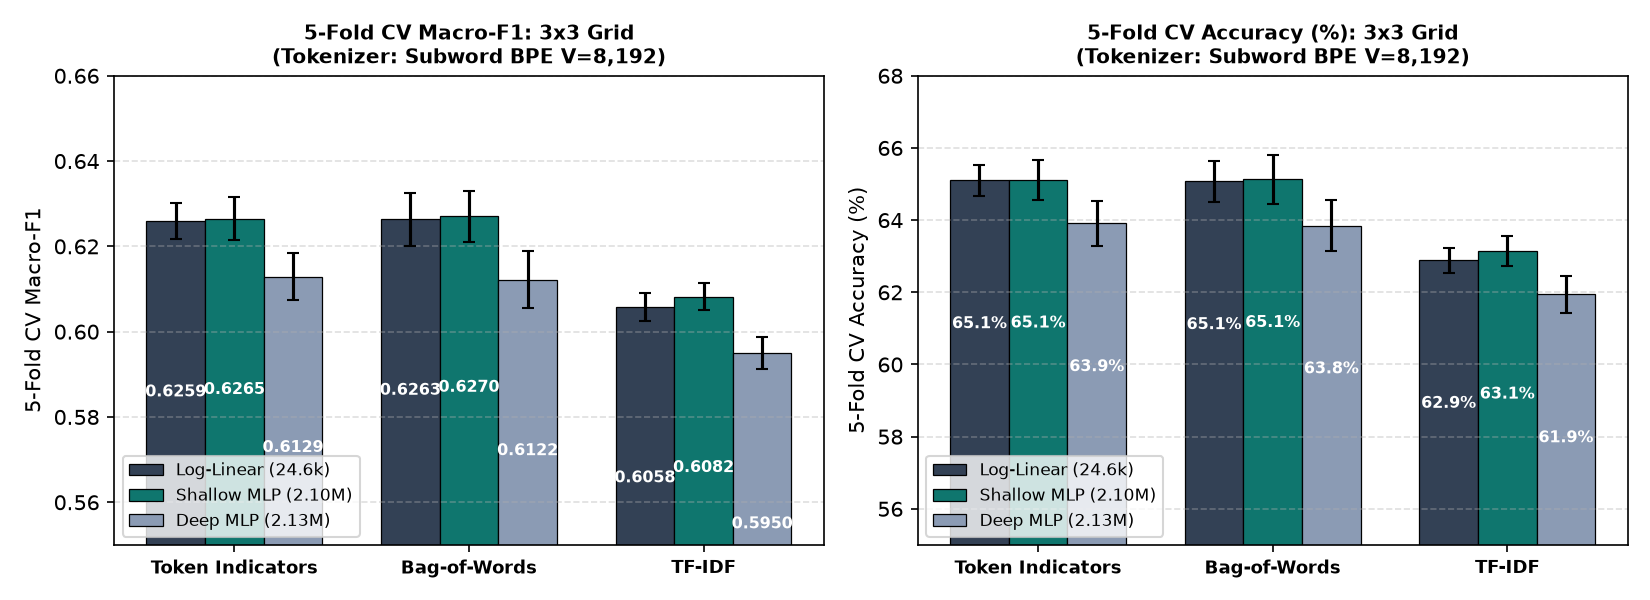
\includegraphics[width=0.98\textwidth]{figures/fig4_cv_grid_results.png}\\[1mm]
    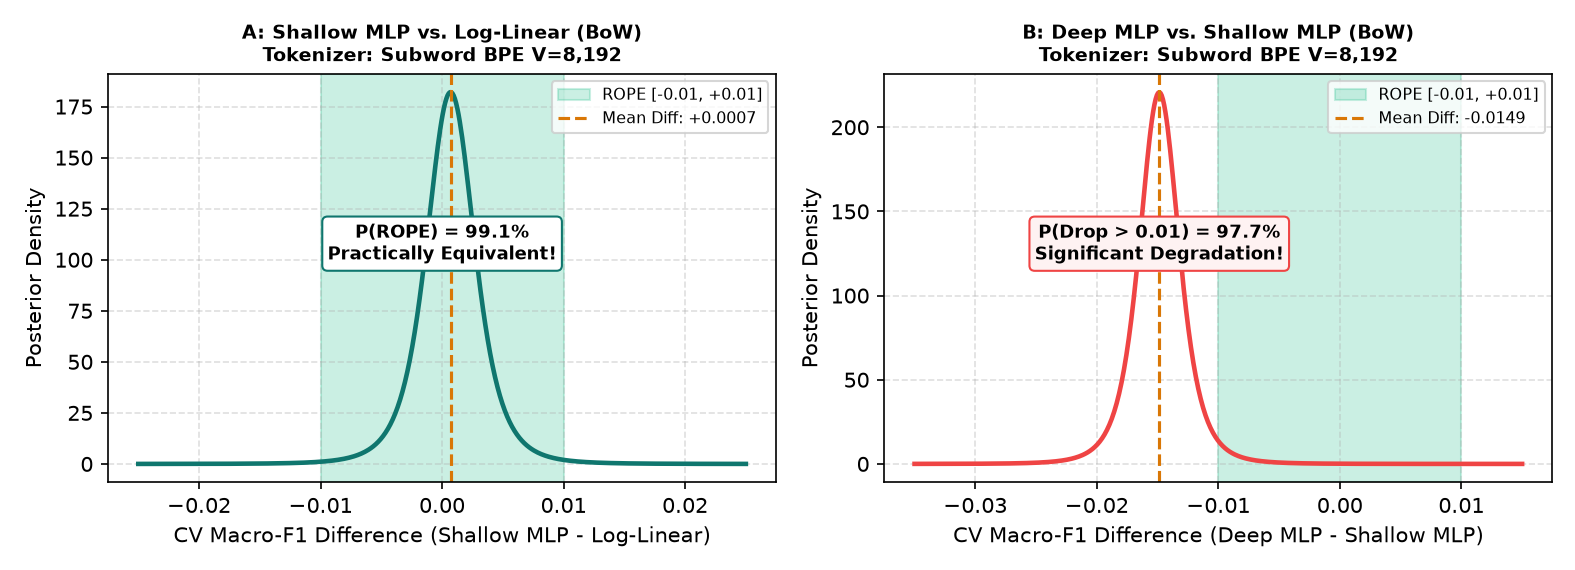
\includegraphics[width=0.98\textwidth]{figures/fig5_bayesian_rope_posteriors.png}
  \end{column}
\end{columns}
\end{frame}

% ==============================================================================
% SLIDE 6: OFFICIAL TEST SET EVALUATION & ERROR ANALYSIS (TOPIC 6)
% ==============================================================================
\begin{frame}{6. Official Test Set ($N = 12,284$) \& Lecture 2a Error Analysis}
\vspace{-2mm}
\begin{columns}[T, onlytextwidth]
  \begin{column}{0.48\textwidth}
    \begin{block}{Official Held-Out Test Set Performance (BPE $V = 8,192$)}
      \scriptsize
      \centering
      \renewcommand{\arraystretch}{1.02}
      \resizebox{\textwidth}{!}{%
      \begin{tabular}{@{}llcccc@{}}
        \toprule
        \textbf{Model} & \textbf{Representation} & \textbf{Params} & \textbf{CV F1} & \textbf{Test Macro-F1} & \textbf{Test Accuracy} \\
        \midrule
        Log-Linear & Token Indicators & $24,579$ & $0.6259$ & $0.5791$ & $58.85\%$ \\
        \rowcolor{rowteal} \textbf{Log-Linear} & \textbf{Bag-of-Words} & $\mathbf{24,579}$ & $\mathbf{0.6263}$ & $\mathbf{0.5799}$ & $\mathbf{58.91\%}$ \\
        Log-Linear & TF-IDF & $24,579$ & $0.6058$ & $0.5584$ & $56.72\%$ \\
        \rowcolor{rowteal} \textbf{Shallow MLP} & \textbf{Bag-of-Words} & $\mathbf{2,098,179}$ & $\mathbf{0.6270}$ & $\mathbf{0.5862}$ & $\mathbf{59.46\%}$ \\
        Deep MLP & Bag-of-Words & $2,130,691$ & $0.6122$ & $0.5695$ & $57.88\%$ \\
        \bottomrule
      \end{tabular}}
    \end{block}
    \vspace{-2mm}
    \begin{alertblock}{3 Concrete Error Modes Linked to Lecture 2a Challenges}
      \scriptsize
      \begin{enumerate}\setlength{\itemsep}{1pt}
        \item \textbf{Negation Scope (\textit{Uninformative Representations})}: \texttt{"...isn't so bad"} (True: \textbf{Neu}) $\to$ Log-Linear predicts \textbf{Pos} (\texttt{"interesting"}), Shallow MLP predicts \textbf{Neg} (\texttt{"vulnerability"}). Neither links \texttt{"isn't"} to \texttt{"bad"} without word order.
        \item \textbf{Topic Bias (\textit{Spurious Correlation})}: Factual news with \texttt{\#Palestine \#Israel} (True: \textbf{Neu}) $\to$ Both predict \textbf{Neg} due to negative training prior on geopolitical hashtags.
        \item \textbf{Sarcasm (\textit{Arbitrariness of Argmax})}: \texttt{"Wow... You always pick the right heroes"} (True: \textbf{Neg}) $\to$ Both predict \textbf{Pos} ($p > 0.78$) on literal \texttt{"Wow"}/\texttt{"heroes"}.
      \end{enumerate}
    \end{alertblock}
  \end{column}
  \begin{column}{0.50\textwidth}
    \centering
    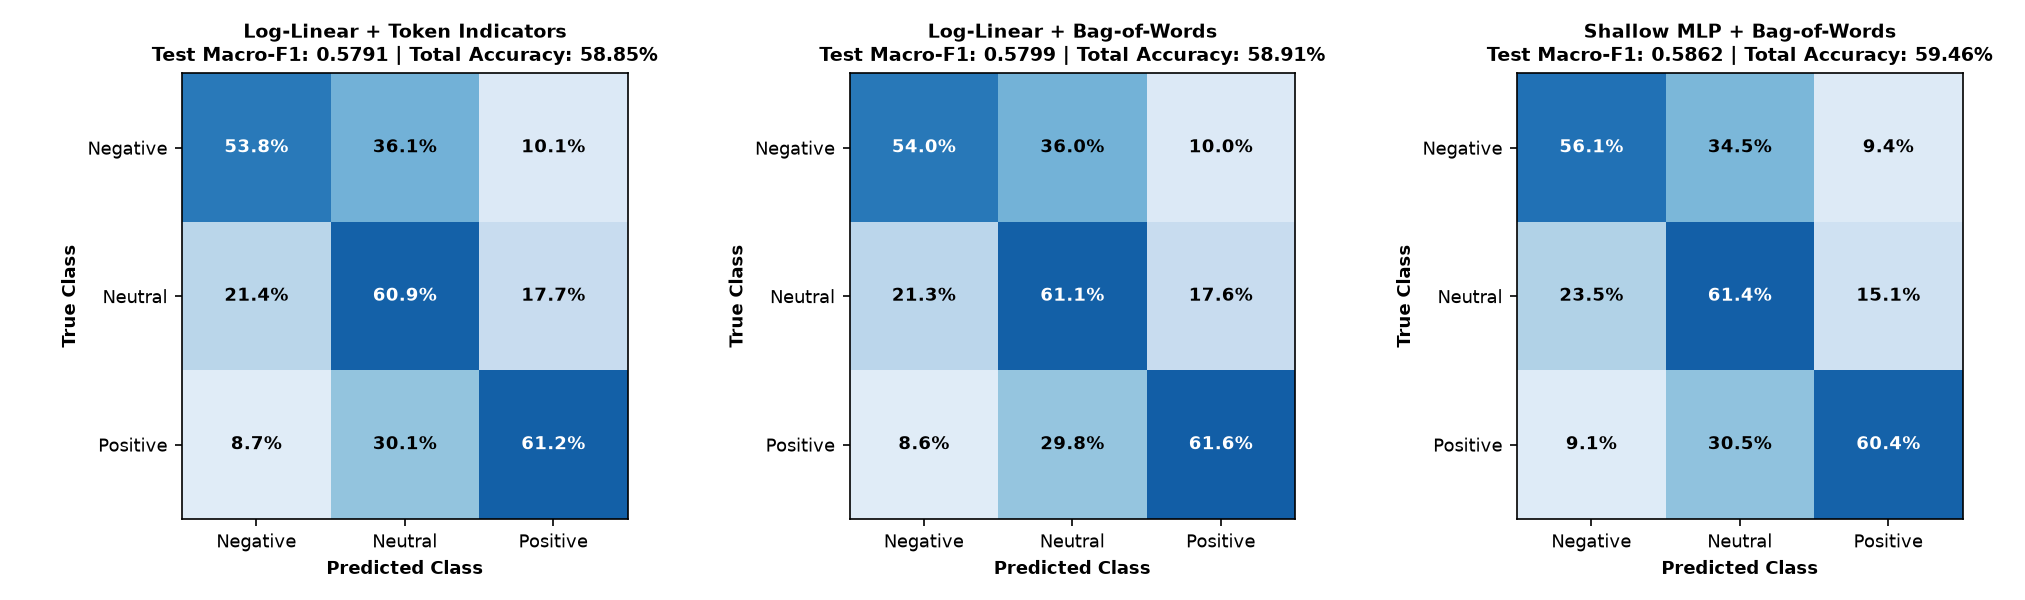
\includegraphics[width=\textwidth]{figures/fig6_test_confusion_matrices.png}
    \vspace{-1mm}
    \begin{exampleblock}{Key Takeaway from Confusion Matrices}
      \scriptsize
      All CV rankings hold on the $12,284$ test tweets: \textbf{Indicators $\approx$ BoW $>$ TF-IDF} and \textbf{Shallow MLP $\approx$ Log-Linear $>$ Deep MLP}. Errors concentrate on the \textbf{Neutral boundary} due to unigram loss of word order and pragmatics.
    \end{exampleblock}
  \end{column}
\end{columns}
\end{frame}

\end{document}
